\section{Linearantennen}

Eine Linearantenne ist ein Typ Antenne, welche eine Länge um die Grösse $\lambda_0/2$ besitzt. Diese werden umgänglich für Mittel- und Langwellen Anwendungen gebraucht wegen ihrer Einfachheit. 

\subsection{Theorie}\label{sec:LinTheo}

Die Antenne besteht aus einem geraden, zylindrischen Leiter, welcher einen dünnen Durchmesser besitzt. Dabei gilt, dass der Schlankheitsgrad

\begin{equation}
s = \frac{l}{d}=\frac{2h}{d} \geq 75
\end{equation} 

beträgt und der Durchmesser

\begin{equation}
d \leq \frac{\lambda_0}{50}
\end{equation}

erfüllt. Somit kann für die Berechnung der Felder die Integration über eine Hüllfläche durch eine eindimensionale Integration vereinfacht werden, was den Rechenaufwand erleichtert.

\begin{figure}[!ht]
	\centering
    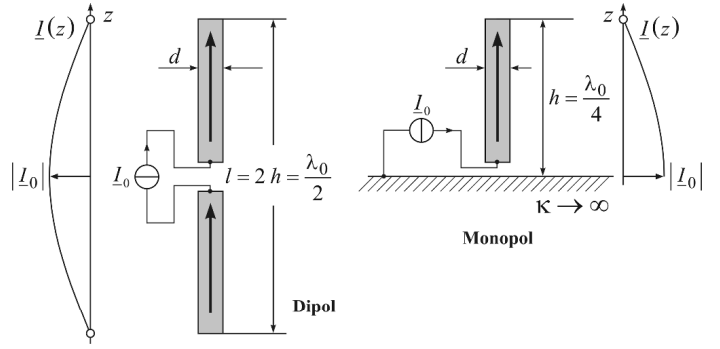
\includegraphics[width=\textwidth]{DiMonopol.png}
    \caption{Unterschiedliche Speisung von Monopol und Dipolantennen.}
    \label{fig:DiMonopol}
\end{figure}

Die lineare Antenne kann auf zwei Arten gespiesen werden. Entweder wird die Antenne als Monopol betrieben und am Fusspunkt gegen Erde erregt, oder sie wird in der Mitte als Monopol symmetrisch erregt (dargestellt in Abbildung \ref{fig:DiMonopol}). Bei der Dipol Ausführung ist jedoch ein Spalt in der Mitte notwendig, welcher vernachlässigbar klein sein soll. Die beiden Anordnungen unterscheiden sich nicht im Strahlungsdiagramm da die Erdoberfläche die Symmetrieebene des elektrischen Feldes darstellt. Der Monopol, welcher halb so lang wie der Dipol gewählt wird, gibt bei einem identischen Speisestrom gerade die halbe Strahlungsleistung ab, was zu einem doppelten Gewinn führt.\\

Für die Simulationen interessieren uns die Richtdiagramme der Linearantennen. Dazu wurde der Halbwellendipol, der Ganzwellendipol und der Doppelwellendipol betrachtet. Die Herleitung der Richtcharakteristik wurde weggelassen, da uns hauptsächlich die Simulationsresultate interessieren. Die bereits berechneten Werte wurden aus dem Buch von K. Kark entnommen \cite{book}.\\

Der Halbwellendipol besitzt eine Antennenlänge von $\lambda_0/2$, was zu einer Richtcharakteristik von 

\begin{equation}\label{eq:RichtHalb}
C(\vartheta) = \frac{\cos \left(\frac{\pi}{2}\cos \vartheta \right)}{\sin \vartheta}
\end{equation}

führt. Die Richtcharakteristik des Ganzwellendipols beträgt bei dessen Antennenlänge von $\lambda_0$

\begin{equation}
C(\vartheta) = \frac{\cos^2 \left(\frac{\pi}{2}\cos \vartheta \right)}{\sin \vartheta}.
\end{equation}

Der Doppelwellendipol ist $2\lambda_0$ lang und dessen Richtcharakteristik beträgt

\begin{equation}\label{eq:RichtDoppel}
C(\vartheta) = \frac{\sin^2 \left(\pi \cos \vartheta \right)}{\sin \vartheta}.
\end{equation}

\begin{figure}[!ht]
	\centering
    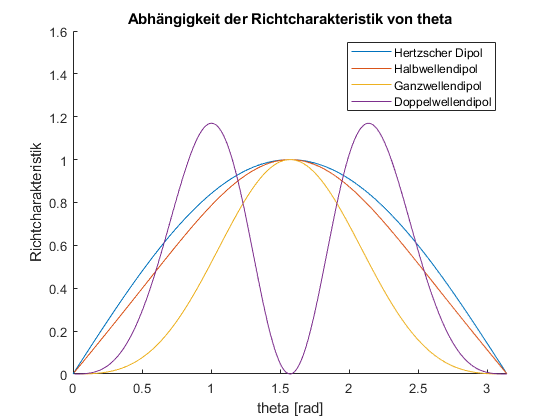
\includegraphics[width=\textwidth/4*3]{Wellendipol.png}
    \caption{Ein Plot der jeweiligen Richtcharakteristiken verschiedener Linearantennen.}
    \label{fig:Wellendipol}
\end{figure}

In Abbildung \ref{fig:Wellendipol} ist die Richtcharakteristik der Antennen in Abhängigkeit von $\vartheta$ zu sehen. Dabei wurde der Hertzsche Dipol auch eingefügt, um die Richtdiagramme besser vergleichen zu können. Wie sich erkennen lässt, besitzt der Hertzsche Dipol die grösste Halbwertsbreite von allen Antennen. Beim Halbwellendipol ist diese nur leicht kleiner, wobei sich beim Ganzwellendipol eine bemerkbar kleinere Halbwertsbreite einstellt. Dabei liegen die -3dB Punkte bei \num{1.99} und \num{1.15}, welche eine Halbwertsbreite von \SI{48}{\degree} besitzen. Diese beträgt fast halb so viel wie die \SI{90}{\degree} Halbwertsbreite des Hertzschen Dipols. Der Doppelwellendipol besitzt sogar eine Nullstelle bei $\pi/2$, wo sich die Maximalwerte der anderen Antennen befinden. Der Maximalwert des Doppelwellendipols liegt jedoch bei \num{1} und \num{2.14}, was einen Maximalwert bei \SI{57.3}{\degree} und \SI{122.6}{\degree} ergibt. Dabei wird klar, dass das dazugehörige Richtdiagramm vier Keulen besitzen wird.\\

\subsection{Simulation}

Im Buch von K. Kark auf Seite 249 befindet sich eine Tabelle mit den Richtdiagrammen der obigen genannten linearen Antennen \cite{book}. Dabei wurde die Länge der jeweiligen Antenne noch mit dem Faktor n angepasst, was uns aus den Formeln \ref{eq:RichtHalb} bis \ref{eq:RichtDoppel} folgende Längen und Richtcharakteristiken ergeben:

Für den Halbwellendipol:

\begin{align}
l &= (2n-1)\frac{\lambda_0}{2}\label{eq:l1}\\
C(\vartheta) &= \frac{\cos \left(\frac{2n-1}{2}\pi \cos \vartheta \right)}{\sin \vartheta}
\end{align} 

Für den Ganzwellendipol:

\begin{align}
l &= (2n-1)\lambda_0\label{eq:l2}\\
C(\vartheta) &= \frac{\cos^2 \left(\frac{2n-1}{2}\pi \cos \vartheta \right)}{\sin \vartheta}
\end{align} 

Für den Doppelwellendipol:

\begin{align}
l &= 2n\lambda_0\label{eq:l3}\\
C(\vartheta) &= \frac{\sin^2 \left(n \pi \cos \vartheta \right)}{\sin \vartheta}
\end{align} 

Für die Simulation wurde ein Dipol mit anpassbarer Länge aufgebaut, mit welchem zwischen den drei in den Formeln \ref{eq:l1}, \ref{eq:l2} und \ref{eq:l3} genannten Längen umgeschaltet werden kann. Für die Anregung sitzt ein Vakuum mit vernachlässigbarer Länge in der Mitte der Antenne, in welchem sich der Anregungsport befindet. Für die Simulation wurde das Standard Anregungssignal verwendet und als Frequenz wurde \SI{1}{\giga\hertz} verwendet. Die Datei wurde so geschrieben, dass alle Antennentypen mit minimalem Aufwand simuliert werden können, ohne dass das Modell abgeändert werden muss. Für alle Abbildungen wurde der Vertikalschnitt der Richtcharakteristik genommen. Es entsteht eine Rotationssymmetrie auf der Antennenachse (was in der Simulation der z-Achse entspricht).

\newpage

\begin{figure}[!ht]
	\centering
    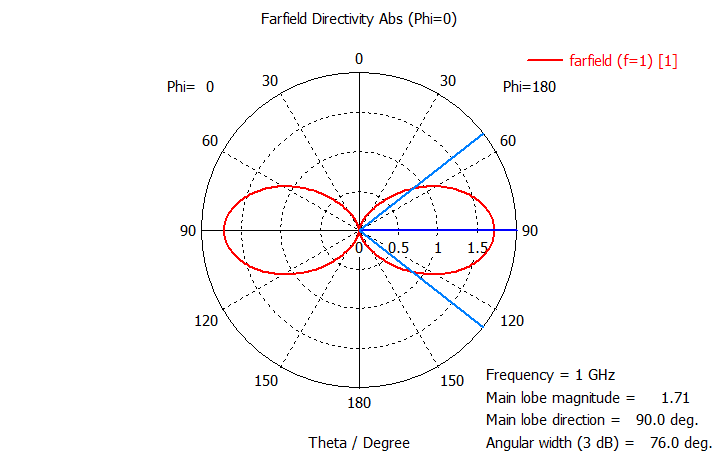
\includegraphics[width=\textwidth]{Halbwellendipol1.png}
    \caption{Direktivität der Halbwellendipolantenne.}
    \label{fig:Halbwellendipol1}
\end{figure}

In Abbildung \ref{fig:Halbwellendipol1} ist das Richtdiagramm des Halbwellendipols zu sehen. Wie bereits erwähnt ist dessen Halbwertsbreite leicht kleiner als \SI{90}{\degree} welche bei $\vartheta = 90^\circ$ am stärksten abgestrahlt wird.

\begin{figure}[!ht]
	\centering
    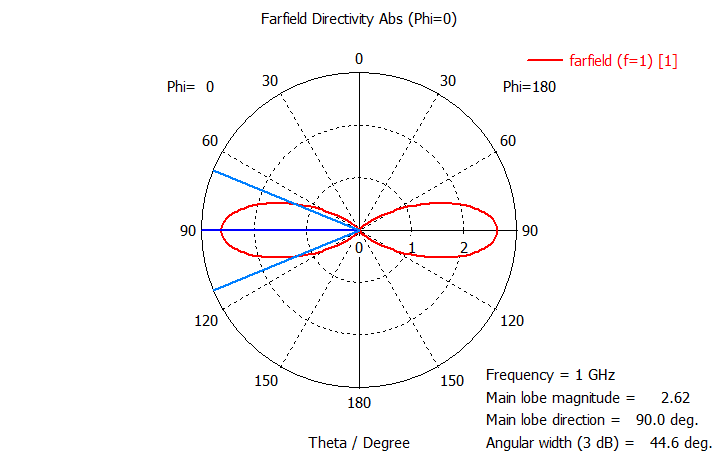
\includegraphics[width=\textwidth]{Ganzwellendipol1.png}
    \caption{Richtdiagramm des Ganzwellendipoles.}
    \label{fig:Ganzwellendipol1}
\end{figure}

Abbildung \ref{fig:Ganzwellendipol1} zeigt die Direktivität des Ganzwellendipols. Berechnet wurde dabei eine Halbwertsbreite von \SI{48}{\degree} und simuliert wurde eine Halbwertsbreite von \SI{44.6}{\degree}. Diese Abweichung ist minimal, weshalb die Simulation als erfolgreich verifiziert werden kann. Auch hier ist die Richtung der maximalen Leistungsabgabe identisch mit dem vorherigen Resultat.

\begin{figure}[!ht]
	\centering
    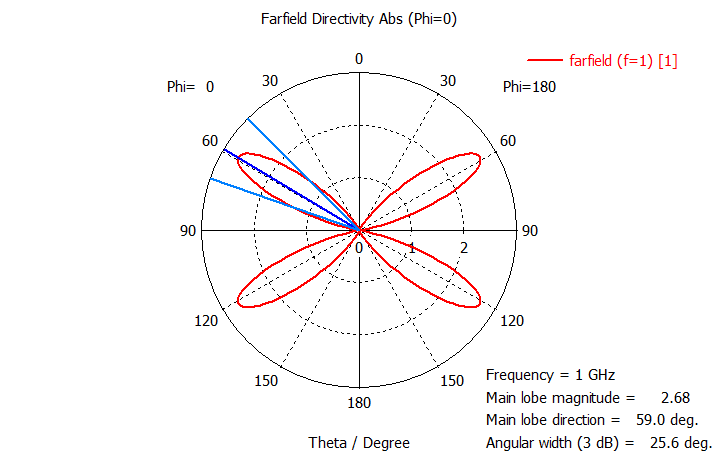
\includegraphics[width=\textwidth]{Doppelwellendipol1.png}
    \caption{Resultat der Simulation des Doppelwellendipols.}
    \label{fig:Doppelwellendipol1}
\end{figure}

Wie in Abbildung \ref{fig:Doppelwellendipol1} zu sehen ist, verhält sich das Richtdiagramm wie im Abschnitt \ref{sec:LinTheo} beschrieben wurde. Es entstehen vier Keulen, wobei der Winkel bei der Simulation \SI{59}{\degree} beträgt anstelle der berechneten \SI{57.3}{\degree}. Dies ist auch wiederum eine vernachlässigbar kleine Abweichung.\\

Als Abschluss der linearen Antenne wurden in Abbildungen \ref{fig:Halbwellendipol13} bis \ref{fig:Doppelwellendipol13} die höheren Ordnungen für $n$ simuliert. 

\newpage

\begin{figure}[!ht]
	\centering
    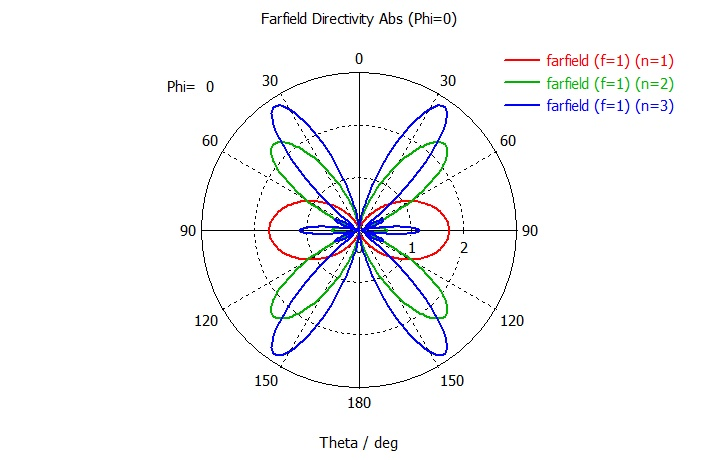
\includegraphics[width=\textwidth]{Halbwellendipol13.jpg}
    \caption{Direktivität der Halbwellendipolantenne mit $n = 1 ... 3$.}
    \label{fig:Halbwellendipol13}
\end{figure}

\begin{figure}[!ht]
	\centering
    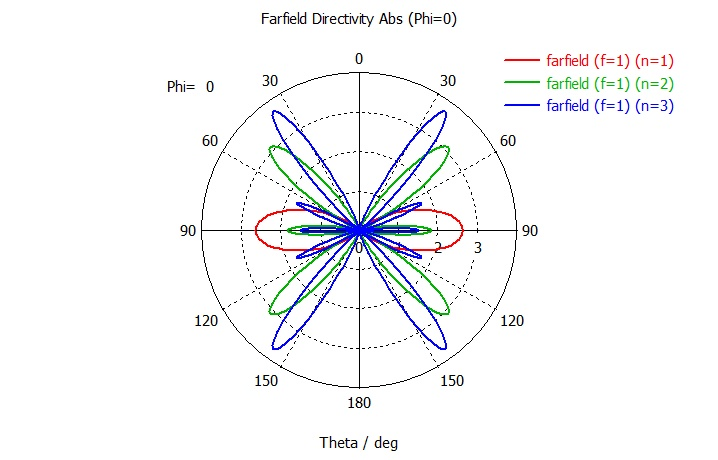
\includegraphics[width=\textwidth]{Ganzwellendipol13.jpg}
    \caption{Richtdiagramm des Ganzwellendipoles mit $n = 1 ... 3$.}
    \label{fig:Ganzwellendipol13}
\end{figure}

\newpage

\begin{figure}[!ht]
	\centering
    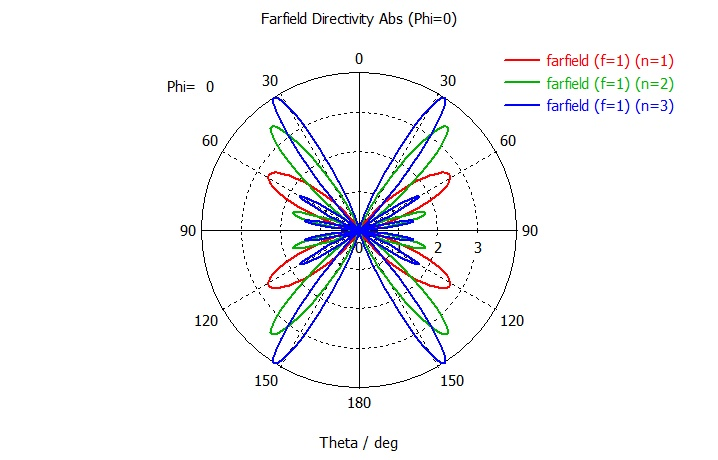
\includegraphics[width=\textwidth/10*9]{Doppelwellendipol13.jpg}
    \caption{Resultat der Simulation des Doppelwellendipols mit $n = 1 ... 3$.}
    \label{fig:Doppelwellendipol13}
\end{figure}

Die Resultate decken sich alle mit der Theorie des Fachbuches. Die Anzahl Seitenkeulen steigt identisch mit den im Fachbuch beschriebenen Abbildungen wenn die Ordnung $n$ vergrössert wird, wobei ab einer Länge grösser als $\lambda_0$ Seitenkeulen entstehen. Diese entstehen durch Überlagerungen von Beiträgen der Elementarstrahlern.

\begin{figure}[!ht]
	\centering
    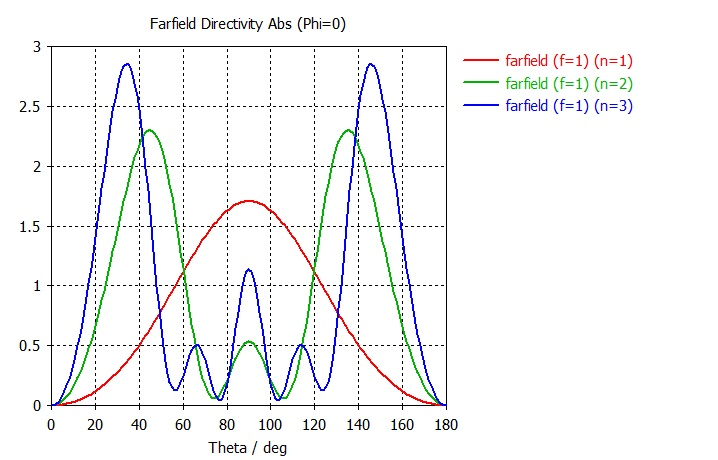
\includegraphics[width=\textwidth/10*9]{Halbwellendipol13Cart.jpg}
    \caption{Direktivität der Halbwellendipolantenne mit $n = 1 ... 3$ in kartesischen Koordinaten.}
    \label{fig:Halbwellendipol13Cart}
\end{figure}

\newpage

Natürlich kann auch im Vergleich zu Abbildung \ref{fig:Wellendipol} das Resultat in Kartesichen Koordinaten dargestellt werden. Dies resultiert in Abbildung \ref{fig:Halbwellendipol13Cart}. Somit stellt dieser Plot dasselbe Resultat wie Abbildung \ref{fig:Halbwellendipol13} dar, wobei bei den kartesischen Koordinaten das Herauslesen der Halbwertsbreite etwas einfacher ist. Bei den Kugelkoordinaten fällt es hingegen leichter, sich die Abstrahlunsrichtungen vorzustellen.

\begin{figure}[!ht]
	\centering
    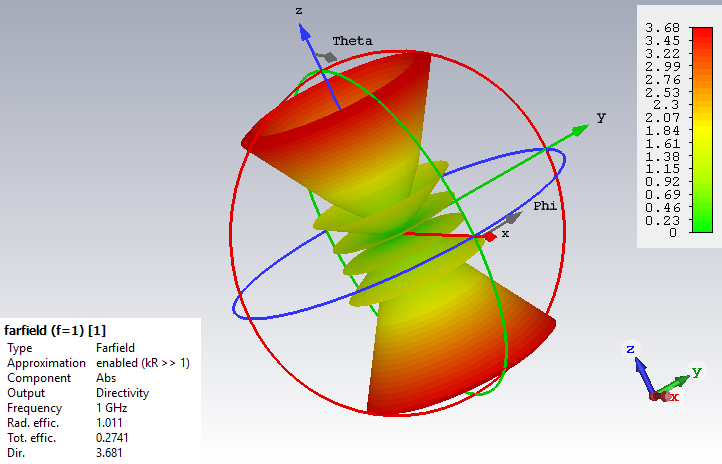
\includegraphics[width=\textwidth]{3D.png}
    \caption{Darstellung des Doppelwellendipols mit $n = 3$ in dreidimensionalen Koordinaten.}
    \label{fig:3D}
\end{figure}

Dabei zeigt Abbildung \ref{fig:3D} die dreidimensionale Direktivität. Es ist ausserdem zu sehen, wie die Antenne geschnitten wurde, um das Richtdiagramm darzustellen (im Vertikalschnitt). Wichtig zu wissen ist, dass verschiedene Antennen in andere Richtungen abstrahlen und daher der Schnittwinkel angepasst werden muss (vergleichsweise Hetzscher Dipol entlang der verschiedenen Achsen in Abschnitt \ref{sec:HerDip}).